\section{PowerGraph}
PowerGraph\cite{PowerGraph} accommodates a sequential greedy heuristic which places the next edge on the machine that minimizes the conditional expected replication factor. The steps are simple.  If A(u) and A(v) are adjacencies of u and v respectively,

Case 1: If A(u) and A(v) intersect, then the edge should be assigned to a machine in the intersection.

Case 2: If A(u) and A(v) are not empty and do not intersect, then the edge should be assigned to one of the machines from the vertex with the most unassigned edges.

Case 3: If only one of the two vertices has been assigned, then choose a machine from the assigned vertex.

Case 4: If neither vertex has been assigned, then assign the edge to the least loaded machine.

\section{Linear Deterministic Greedy}
This consider two important factors when  assigning a vertex to a partition.  They are, how related a vertex to other vertices in a given partition and the capacity remaining in the partition. P\textsuperscript{t}\textsubscript{i}  denotes the ith partition in the given time t, C\textsubscript{i} denotes the capacity of the i\textsuperscript{th} partition. N(u) means the neighbors of vertex u. 

\begin{figure}[H]
\centering
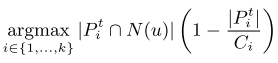
\includegraphics[scale=0.5]{images/image07}
\end{figure}

\section{X-stream}
X-stream\cite{XStream}is proposing streaming partitioning for bounded graphs, that is the vertices and edges remains fixed during the entire computation and the number of partitions stays fixed throughout the computation. The design is motivated by the fact that sequential bandwidth for all storage media (main memory, SSD, etc) is substantially larger than random access bandwidth and a large number of graph algorithms can be expressed using the edge-centric scatter-gather model. 

\paragraph{}

During initialization, the vertex set of the entire graph is partitioned into vertex sets for the different partitions, and the edge list of each partition is computed. 

\section{S-PowerGraph}
S-PowerGraph\cite{S-PowerGraph} discuss several methods as ’Degree’, a greedy procedure which makes use of the in-degree distribution and ’DegreeIO’ which tries to meet the challenge that both indegree and outdegree of natural graphs are skewed. 

\paragraph{}

S-PowerGraph firstly suggests the Grid-based Constrained Random Vertex-cut algorithm of GraphBuilder[?] could be altered for streaming graph partitioning. In this method, a vertex is mapped into a shard which accommodates a constrained set of partitions. Then, the partition a vertex to be assigned will be chosen from the constrained set randomly. The edge e is assigned to P\textsubscript{idx} where idx is decided by idx = GridHash(e), the hash function implemented in GraphBuilder. 

\paragraph{}

Then the S-PowerGraph discuss about an enhanced version of the greedy algorithm proposed in PowerGraph\cite{PowerGraph}. As the greedy algorithm in PowerGraph could lead to some unbalanced partitions in some cases, they introduce Balance(PowerGraph) where Balance() is a constraint to avoid the imbalance.

\paragraph{}

\section{Linear Embedding}
”Distributed Balanced Partitioning via Linear Embedding”\cite{Linear Embedding} discusses a method researchers at Google have tried and tested with Google services. ”Linear Embedding” is a balanced partitioning problem where the goal is to partition the vertices of a given graph into k parts so as to minimize the total cut size. Linear Embedding method first embeds nodes of the graph onto a line, then attempt to improve the ordering mainly by swapping vertices in a semi local manner and finally accommodate a post-processing method to improve the cut-size.

\paragraph{} 

They discuss several different methods for each different step and compare the outcome performances for each combination. For embedding nodes onto a line, they accommodate random mapping, Hilbert curve mapping when geographic/geometric information is available, and Affinity-based mapping which takes into account the affinity of vertices by grouping vertices that are closely connected, hence building a tree of these connections. Once the linear embedding is done, the next step is to improve ordering using semi local moves. One method is using Minimum Linear Arrangement (MinLA)\cite{MinLA} and the other is Rank Swap which depends on the pre chosen cut boundaries, the number of final partitions k.

